\documentclass[12pt]{article}
\usepackage{lingmacros}
\usepackage{tree-dvips}
\usepackage{blindtext}
\usepackage{enumitem}
\usepackage[section]{placeins}
\usepackage{xcolor}
\usepackage{graphicx}
\usepackage{caption}

\graphicspath{{./images/}}


\title{IV3 Clock User Guide}

\begin{document}


\maketitle

\tableofcontents
\newpage

\section{Assembly}
\subsection{Kit Contents}
\begin{description}[font=$\bullet$~\normalfont\scshape]
\item [] Microcontroller PCBA
\item [] Switch PCBA
\item [] Top display PCB
\item [] 4x IV-3 Tubes
\item [] 4x IV-3 breakout PCBs
\item [] 8x 7-pin male headers
\item [] 4x 6mm brass standoff
\item [] 4x 11mm brass standoff
\item [] 4x 16mm brass standoff
\item [] 4x Brass caps 
\end{description}


Your IV-3 Clock kit contains all the components for  your clock, the only things you'll need are a USB-C cable to power it and a CR2032 battery (optionally, but it keeps time while the clock is unplugged).

\subsection{IV-3 Tube assembly}
\renewcommand{\figurename}{Step}

 
\begin{figure}[t]
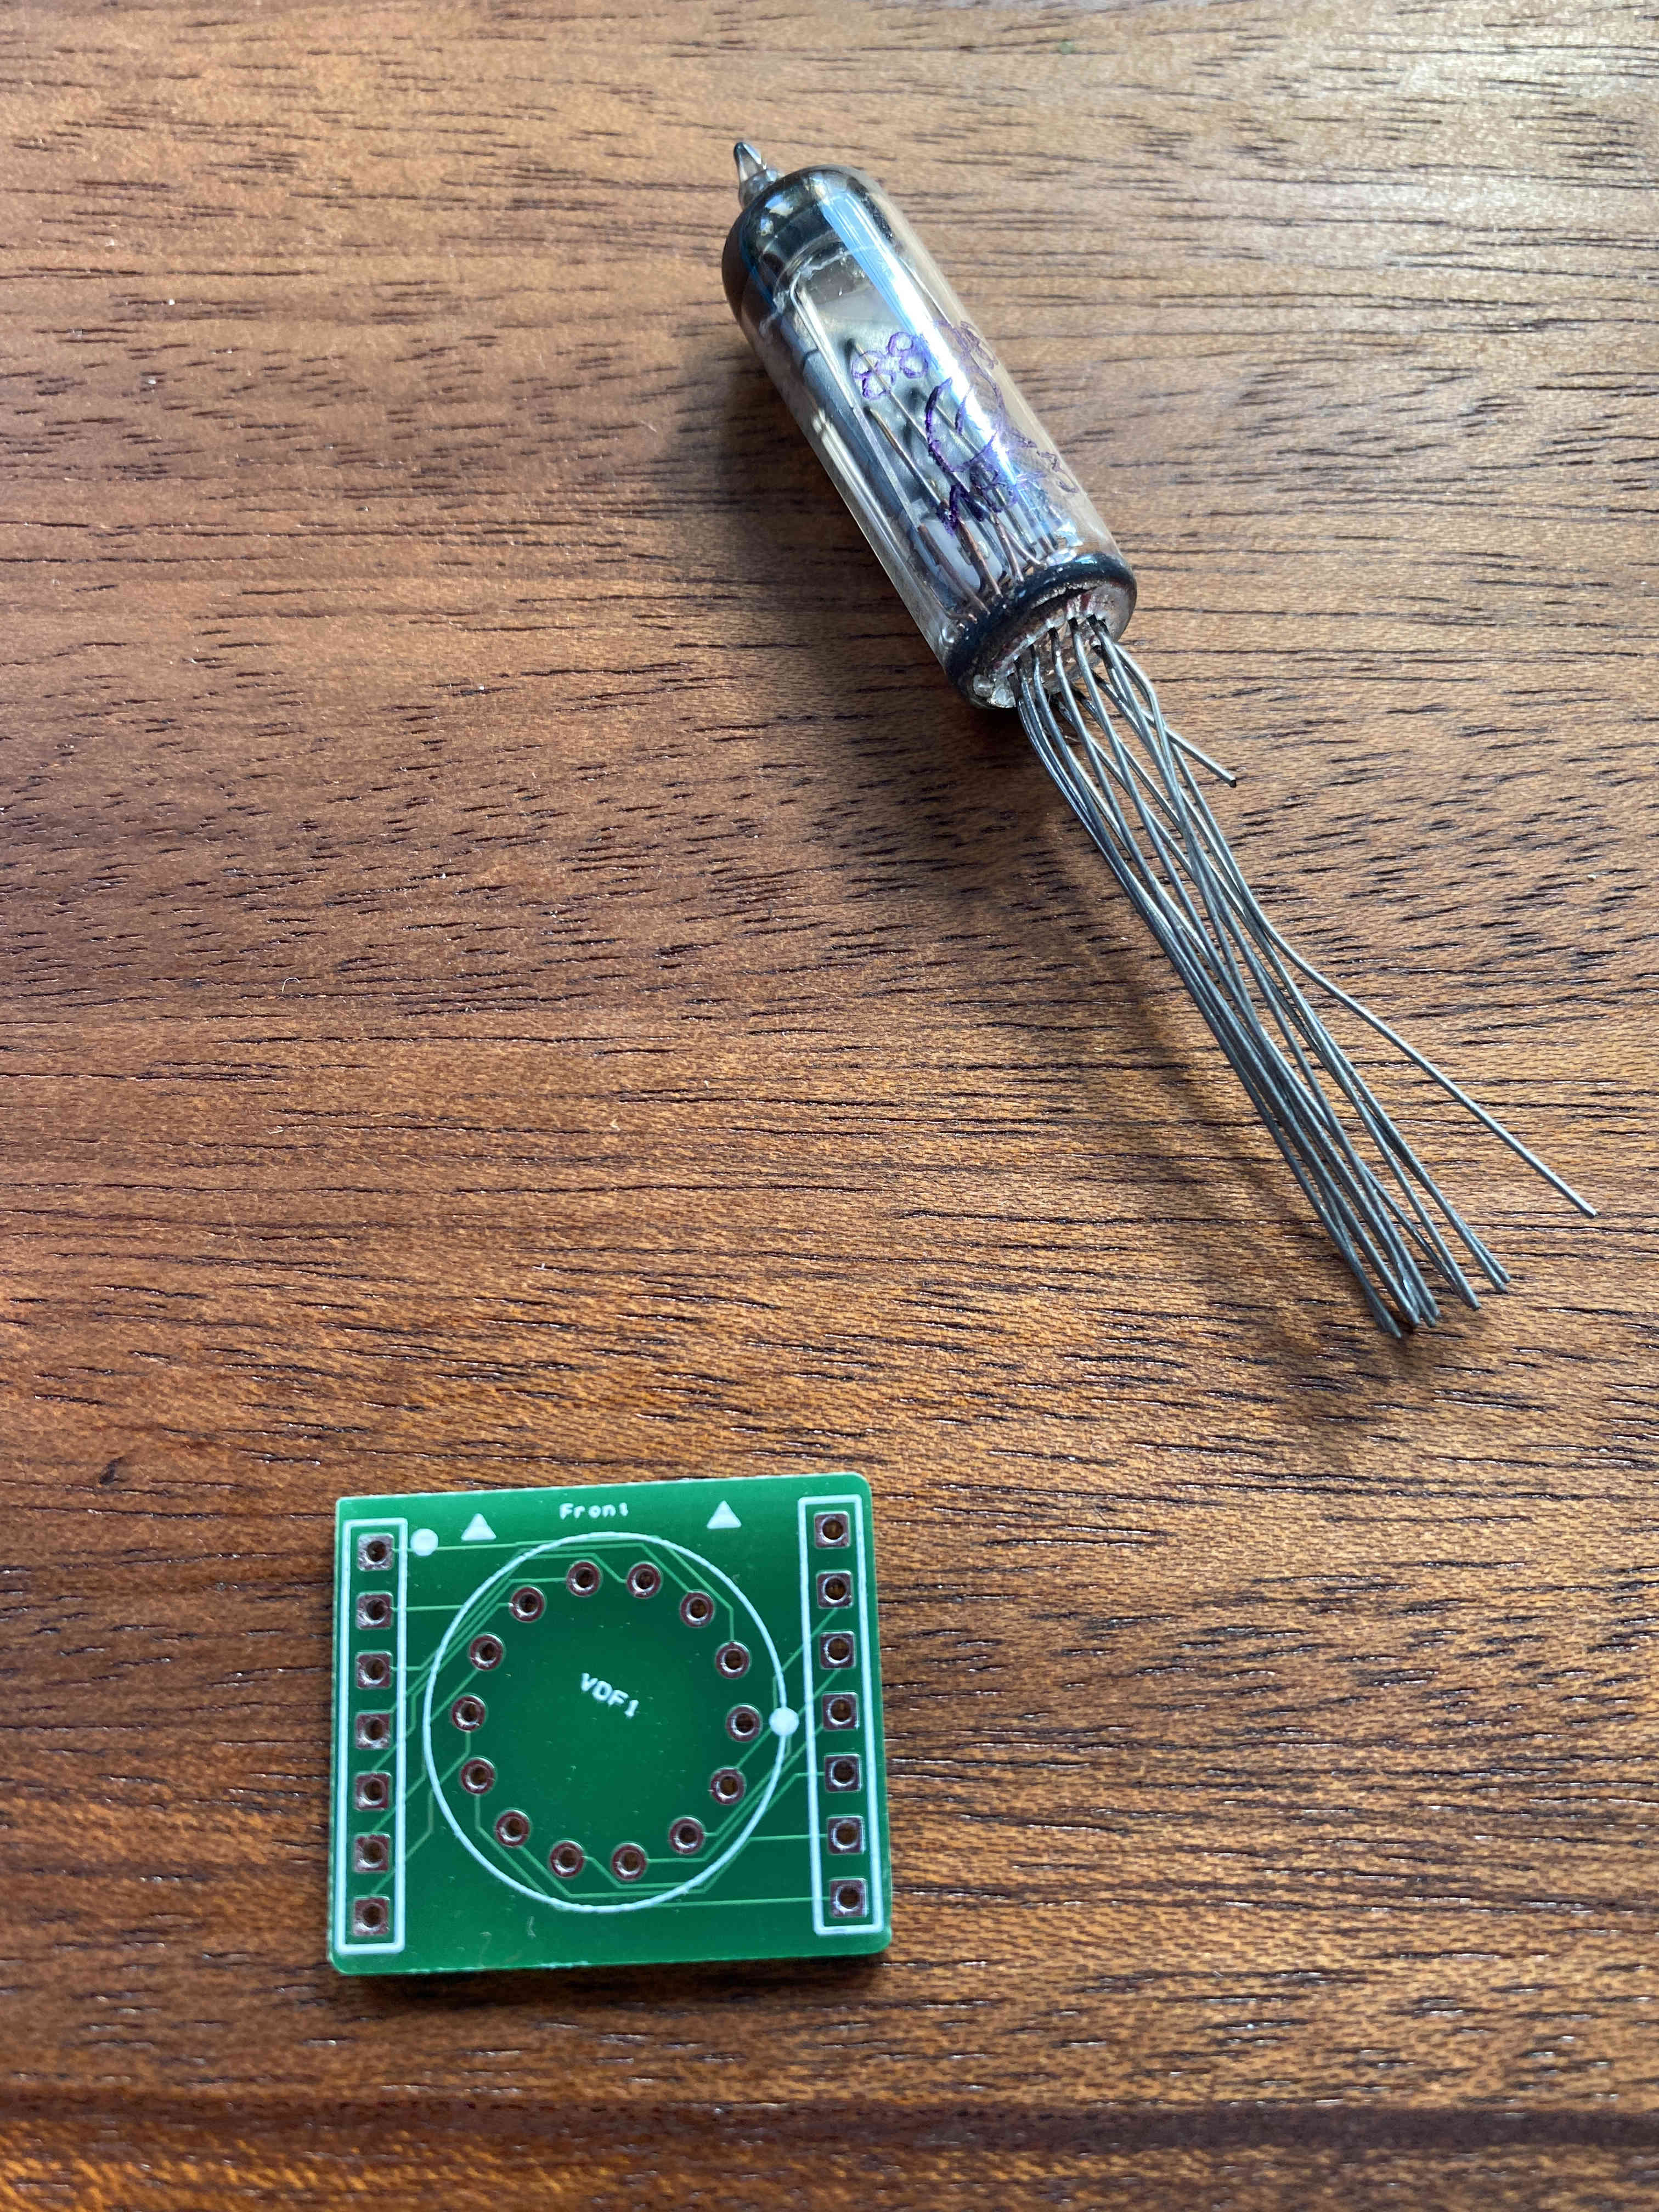
\includegraphics[scale=0.05, angle=270]{IMG_1094}
\centering
\caption{Start by looking at the four small PCBs. On the top you will see along one edge two arrows point to the front of the clock. Next holding a tube, look for the short leg. This leg aligns with the dot on the circle on the PCB. This should align the tube so the face is pointing out to the front of the clock. Carefully, thread all the legs through the holes on the PCB. This can be made easier by shortening the legs, though be careful not to make them too short! Tweezers are also very helpful.}
\label{fig:tubepcb}
\end{figure}

\begin{figure}[t]
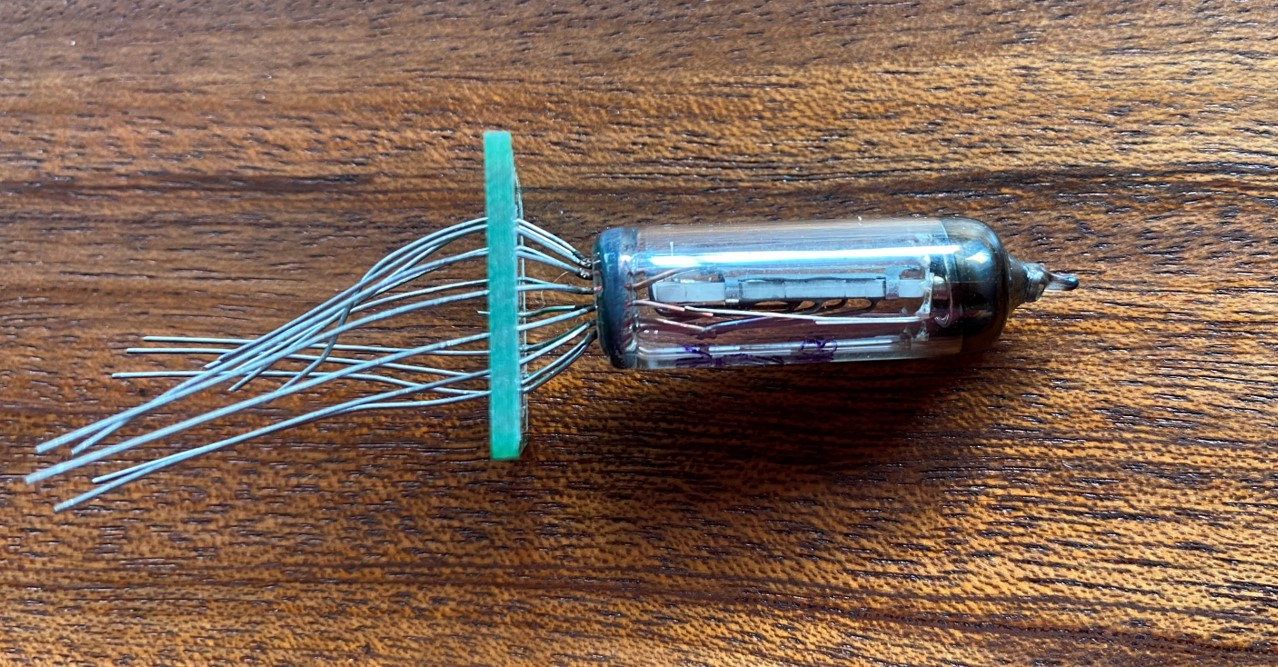
\includegraphics[scale=0.4]{IMG_11051}
\centering
\caption{Once all the legs have been threaded through, pull/push them through until the base of the tube sites about 5mm from the PCB.}
\label{fig:tubeinpcb}
\end{figure}

\begin{figure}[t]
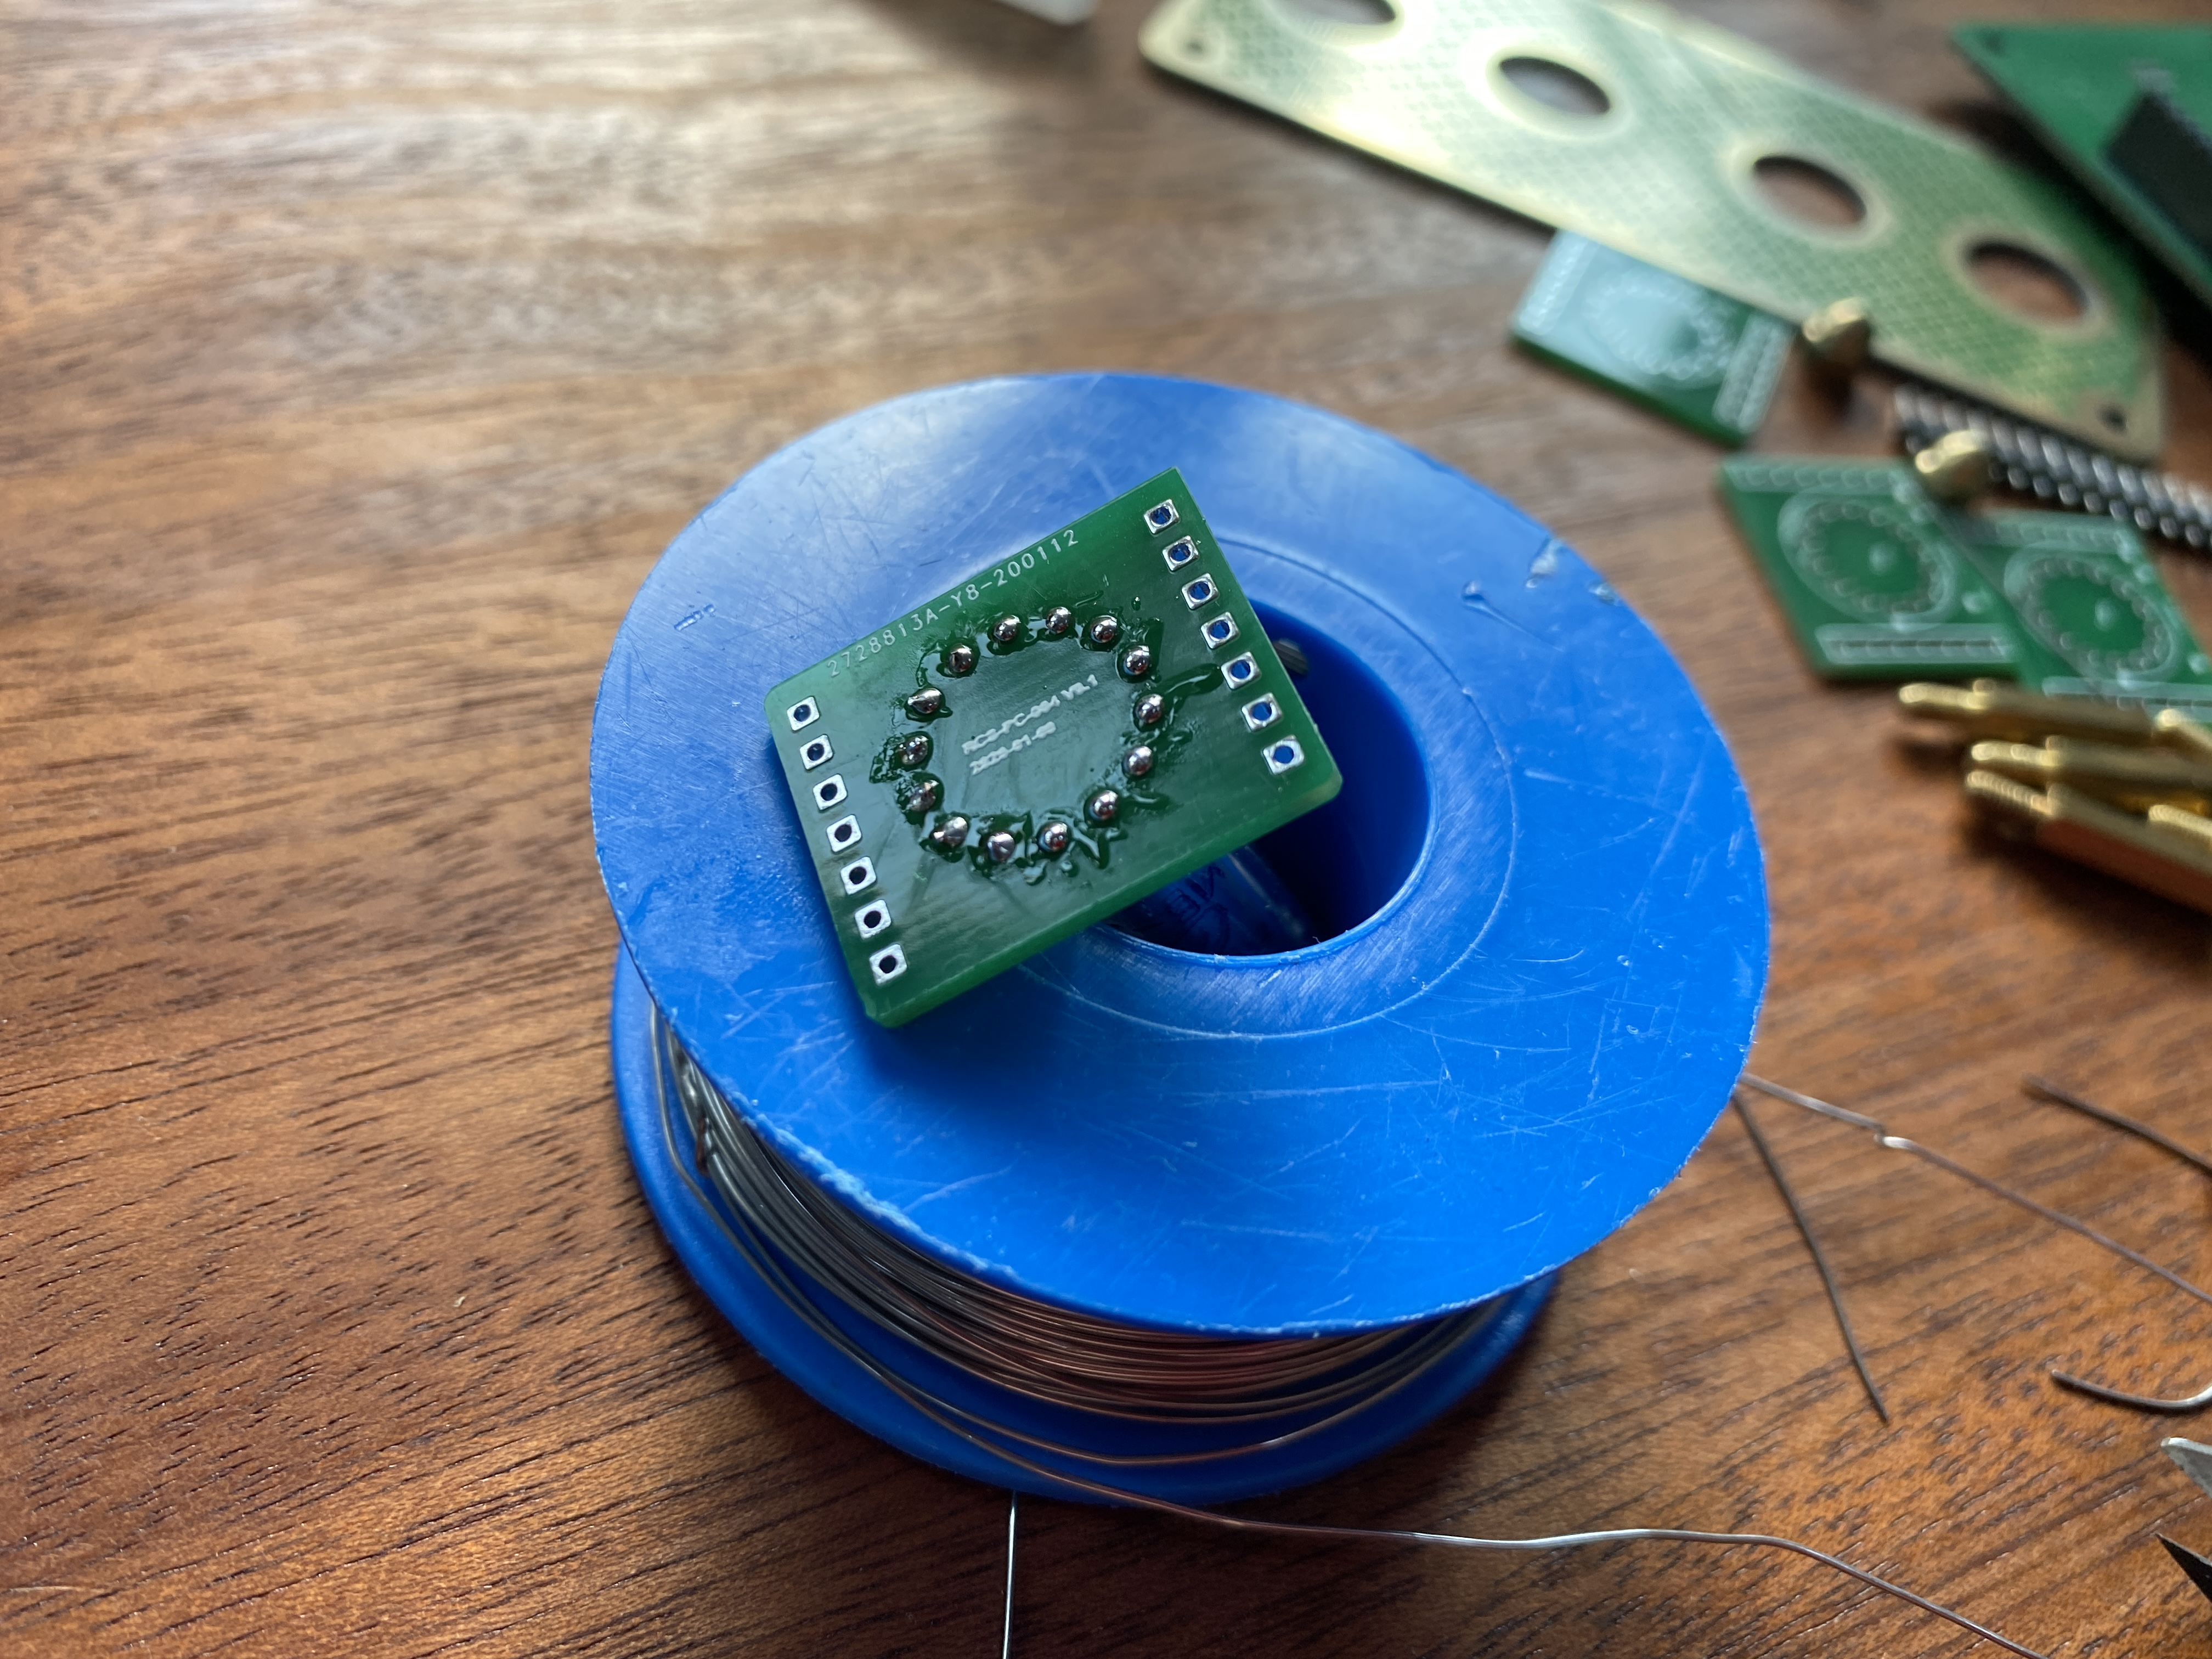
\includegraphics[scale=0.05]{IMG_1109}
\centering
\caption{Solder the legs to the board and trim off the excess.}
\label{fig:tubetrim}
\end{figure}

\begin{figure}[t]
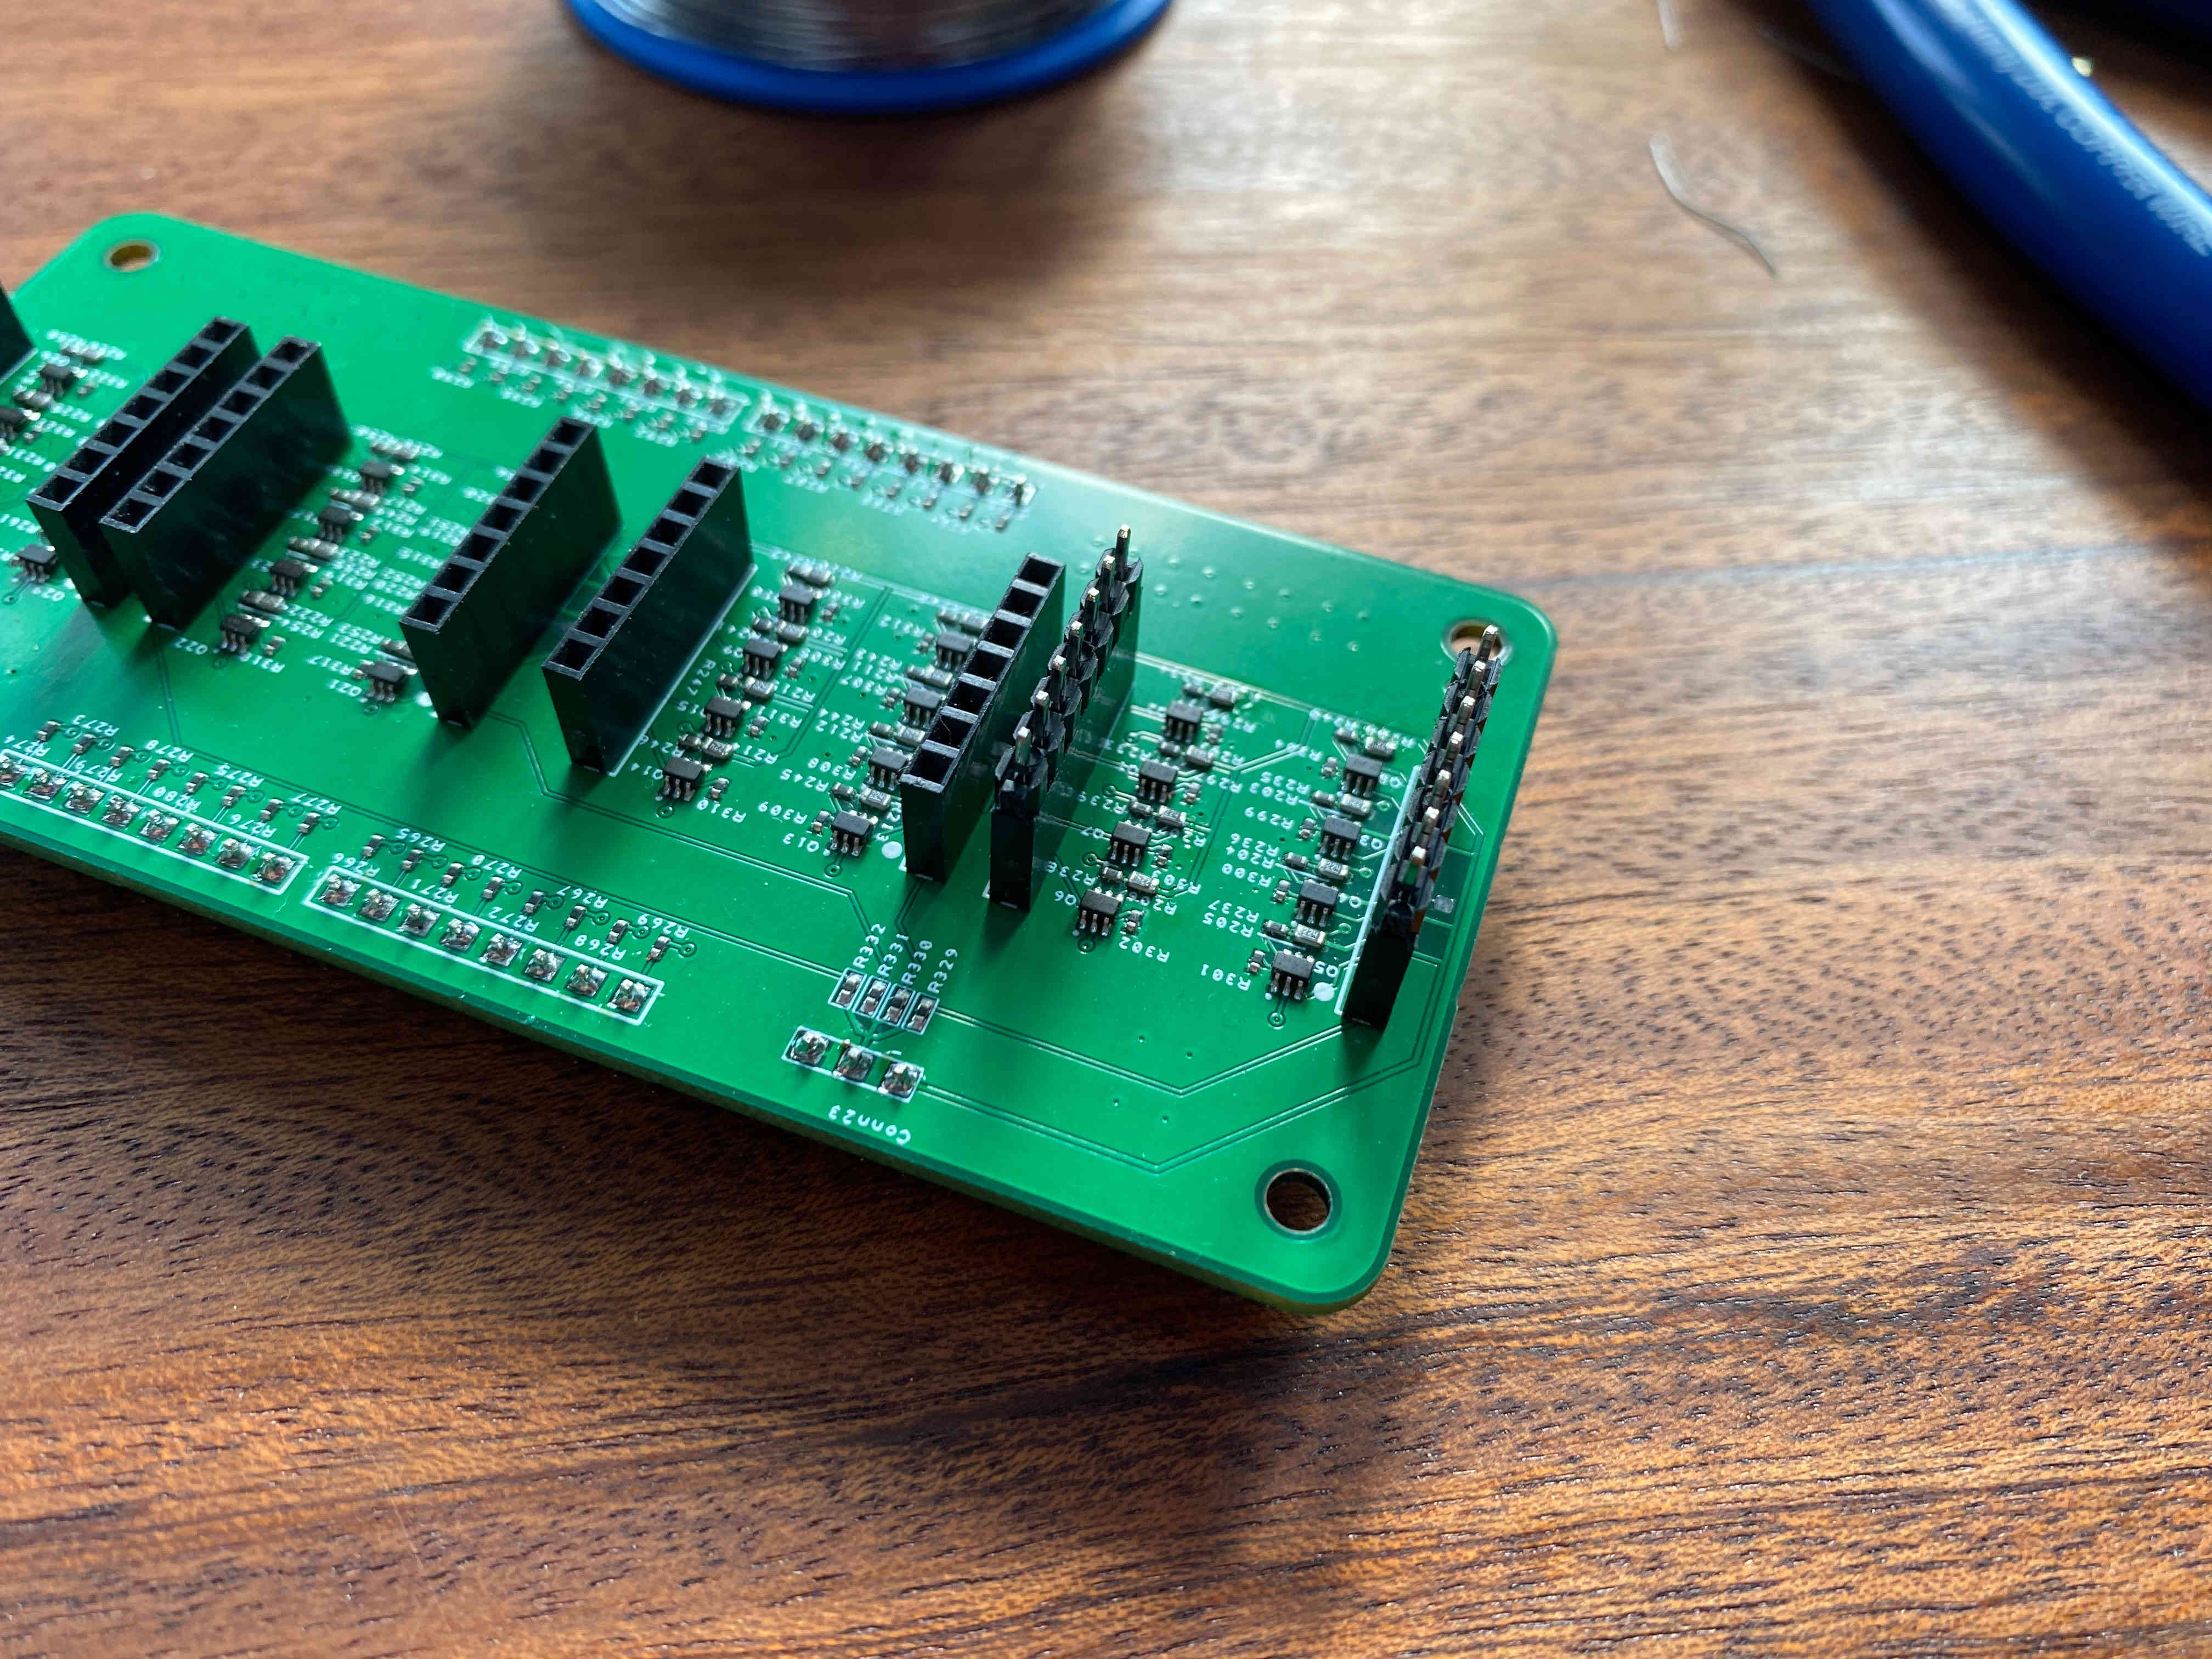
\includegraphics[scale=0.05]{IMG_1111}
\centering
\caption{Place the pin headers in the switch board.}
\end{figure}

\begin{figure}[t]
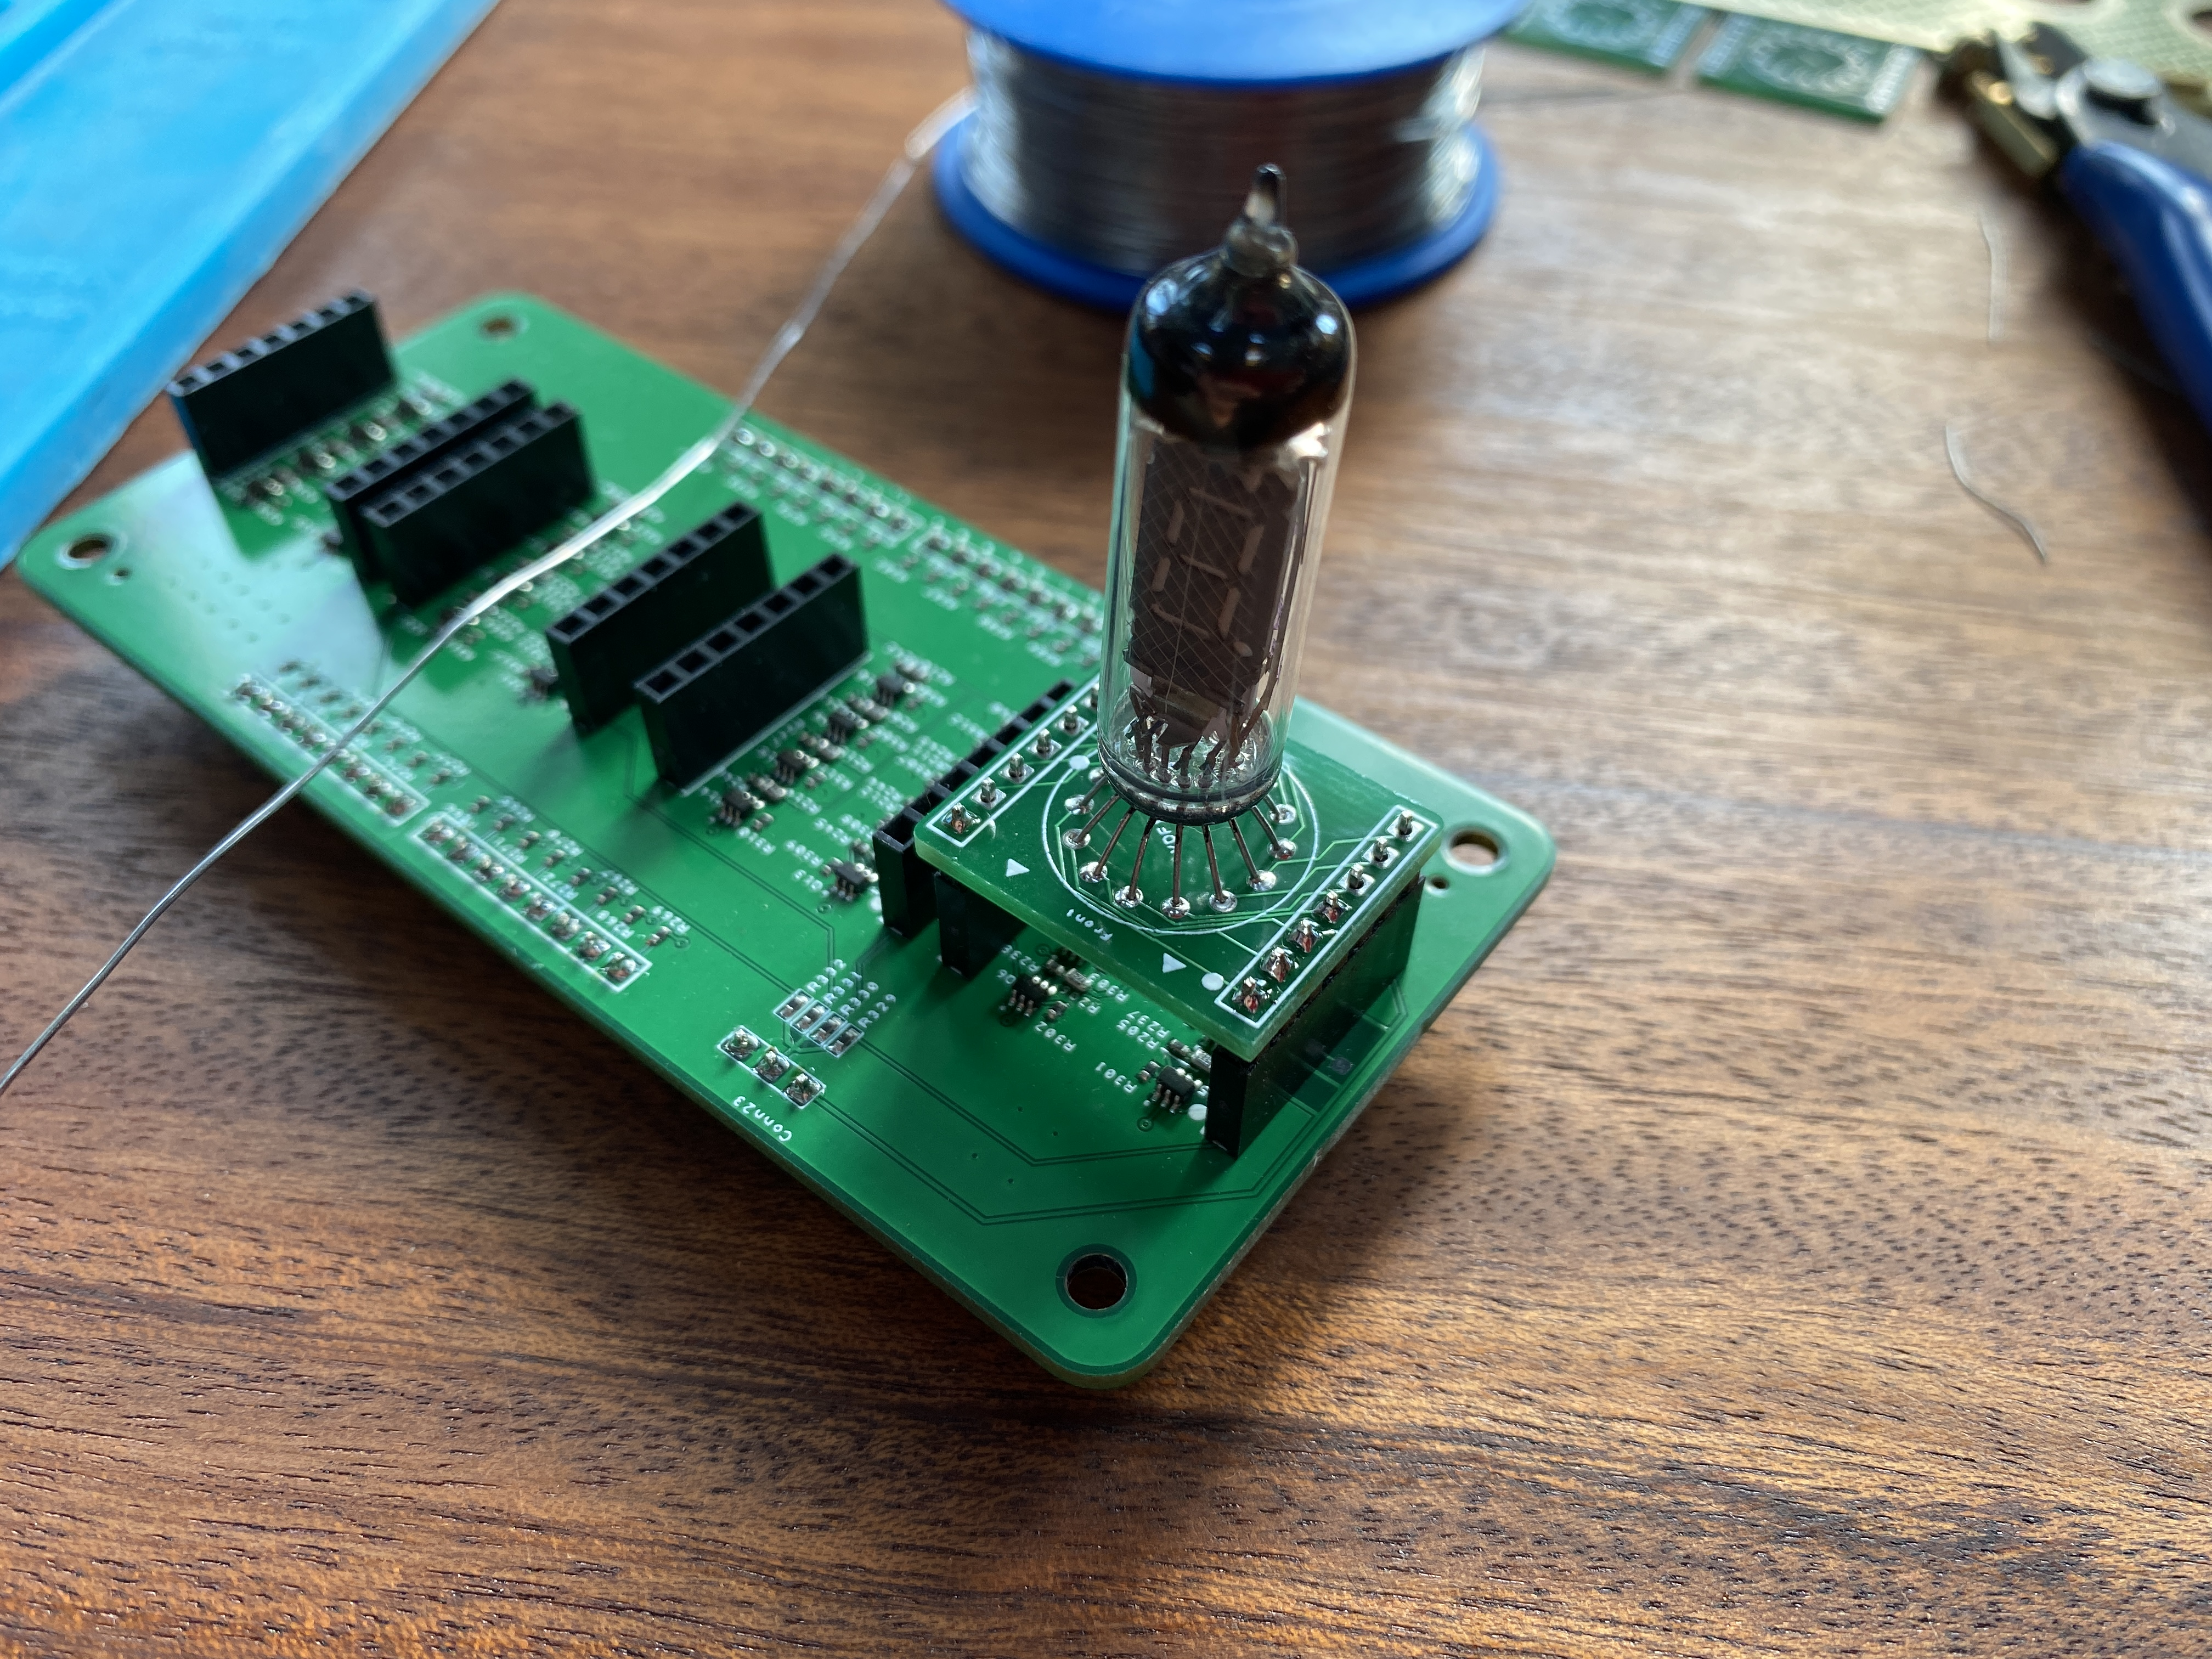
\includegraphics[scale=0.05]{IMG_1113}
\centering
\caption{Mount the tube and breakout board onto the headers and solder into place.}
\end{figure}

\FloatBarrier
\section{Setting the time}
It is very easy to set the clock time. On the underside of the clock there are two buttons labelled Hours and Minutes. These can be used to increment the time. A few notes on setting the time. Holding either button will cause the time to increment, not requiring repeated pushes. When minutes roll over, the hour does not increment. During the hours between 12am and 7am the clock is in a low brightness mode. This is normal but can be turned off in the clock menu (see below). 

\section{Clock menu}
The clock has three settings that can be used to customise your clock.

\begin{description}[font=$\bullet$~\normalfont\scshape]
\item [] 12/24h clock mode
\item [] IV-3 tube brightness
\item [] Night-time dimming
\end{description}

To access the clock menu you press the ``Hours" button twice quickly. The tubes will then stop displaying the time, instead displaying a menu option.

The different menu options can then be selected by single ``Hours" button presses.

To exit the menu simply repeat the double click on the hour button or wait 10 seconds for the menu to time out. On time out all changes to the menu options are saved.

\subsection{Setting 12/24h mode}
You can choose whether the clock displays the time in 12h or 24h mode. Double click the ``Hours" button to access the menu. If the 24h option isn't shown, press the ``Hours" button until it shows. To alternate between ``24h" and ``12h" press the ``Minutes" button. When you have selected the option you like double press the ``Hours" button.

\subsection{Change brightness}
Access the menu and press the ``Hours" button until the brightness option is displayed. By clicking the ``Minutes" button the tube brightness is incrementally decreased. Once the brightness has reached the minimum, the next button press will bring the brightness back to maximum. 

Once you have selected the brightness you like, exit the menu.

\subsection{Night time dimming}
By default the clock dims the tubes to minimum brightness between 12am and 7am. This function can be turned off by opening the ``FAd" menu option. When the last tube displays ``1" then night-time dimming is enabled. Press ``Minutes" and the last tube will switch to ``0", indicating night-time dimming is disabled.

\renewcommand{\figurename}{Fig}

\section{I2C Control}
The clock has been designed to operate as an I2C slave device, enabling control of all the clock functionality as well as complete control of the four tubes. 

The I2C commands available are:
\begin{description}[font=$\bullet$~\normalfont\scshape]
\item [] CMD: 0x00, Set the time
\item [] CMD: 0x01, Read the time
\item [] CMD: 0x02, Clock mode
\item [] CMD: 0x03, User display
\item [] CMD: 0x04, Set 24h/12h mode
\item [] CMD: 0x05, Set brightness
\item [] CMD: 0x06, Set night-time fade
\item [] CMD: 0x07, Get clock status
\item [] CMD: 0x08, Reset
\end{description}

 

\subsection{I2C}
All IV3 clocks share the same address of 0x16. An I2C command must start with the command, followed by the suitable number of bytes. The correct messaging for each command is described below. 
\subsection{Set the time}
This command is used to pass the clock a time which will override the current RTC time. Whilst the clock can only display hours and minutes the RTC also stores the year, month, day and second information. 

To set the time the first byte should be the set time command = 0x00, this is then followed by 6 bytes:

\begin{description}[font=$\bullet$~\normalfont\scshape]
\item [] Byte 0: CMD
\item [] Byte 1: Year
\item [] Byte 2: Month
\item [] Byte 3: Day
\item [] Byte 4: Hour
\item [] Byte 5: Minute
\item [] Byte 6: Second
\end{description}

For example to set the time to 13:45:14 on 18th June 2020 the bytes would be:

\begin{figure}[!h]
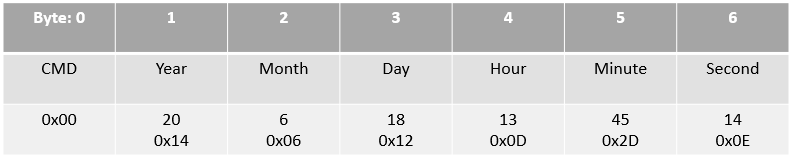
\includegraphics[scale=0.5]{setTime}
\centering
\caption*{}
\label{fig:status}
\end{figure}

\subsection{Read the time}
This command can be used to read the time from the clocks RTC. First write the 1 byte command 0x01 to the clock, followed by read 6 bytes. The bytes are sent from the clock in Year, Month, Day, Hour, Minute, Second order. 

\subsection{Clock mode}
Clock mode command is used to switch from ``User display" back to displaying the time. This command should be used when you no longer want to use it as a display. Simply send the 1 byte command to switch mode. If no user display commands are sent the clock will automatically reset to clock mode after 10 seconds. 

\subsection{User display}
User display command is used to allow you to control what the tubes display. This is done by writing 4 bytes to the clock. Each byte is a bitmask for a tube, with the byte1 for the tube furthest most left tube and working to the right.

\begin{figure}[!h]
\includegraphics[scale=0.1]{7Segment}
\centering
\caption*{}
\label{fig:status}
\end{figure}

Each bit in the byte represents a segment of the display, the least significant bit represents segment A in the figure and the most significant bit DP. 

For example, to write ``3" to a tube you would want to illuminate A, B, C, D and G. Your corresponding bitmask would be 0b01001111 or 0x4F in hex. In the Arduino User Diplay example all the numbers have been defined.

As an example to diplay ``1, 2, 3, 4" on the tubes the bytes you would send would be:
\begin{description}[font=$\bullet$~\normalfont\scshape]
\item [] Byte 0: CMD = 0x03
\item [] Byte 1: 1 = 0x06
\item [] Byte 2: 2 = 0x5B
\item [] Byte 3: 3 = 0x4F
\item [] Byte 4: 4 = 0x66
\end{description}

\subsection{Set 24h/12h mode}
This command can be used to change between 24h and 12h clock modes. Follow the command byte by either a 1 or 0. A 1 sets the clock to 12h mode, while a 0 sets it to 24h mode. 

\subsection{Set brightness}
The tube brightness can be set using this command. The byte following the command corresponds to the brightness. This should be a value between 1 and 20. Brightnesses above 20 will be set the clock to max brightness. 

\subsection{Set night-time fade}
Night-time fade can be controlled with this command. Follow the command byte with a 1 to turn on night-time fade and 0 to turn it off.

\subsection{Get clock status}
This command requests the clock status. After writing the command you should read 1 byte. This byte indicates whether the clock is in 24h or 12h mode, night-time dimming and the current brightness.

\begin{figure}[!h]
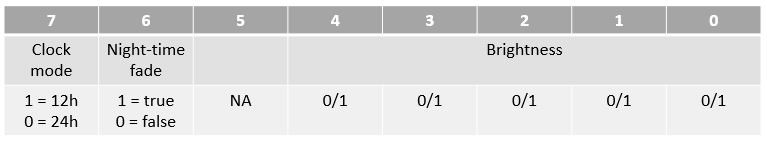
\includegraphics[scale=0.5]{status}
\centering
\caption*{}
\label{fig:status}
\end{figure}


\subsection{Reset}
This command factory resets all the clock setting.

\end{document}